\begin{tikzpicture}

	\onslide<2->{
		\draw[draw=blue!50,fill=cyan!10,thick,solid,rounded corners] (3.2,4.6) rectangle (0.8,7.3);

		\node[inner sep=0pt] (A) at (2,6)
		{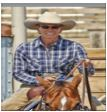
\includegraphics[scale=0.7]{images/CNN_cowboy_scale.JPG}};
	}
	
	\onslide<3->{
		\draw[draw=blue!50,fill=cyan!10,thick,solid,rounded corners] (8.5,4.6) rectangle (3.8,7.3);
		\draw[black, thick, ->]  (3,5.8) --  (4,5.8);
		\node[inner sep=0pt] (C) at (6.2,6) {\begin{tikzpicture}[thick,scale=0.8, every node/.style={scale=0.8}]     
			\pgfsetxvec{\pgfpoint{1cm}{0cm}}
			\pgfsetyvec{\pgfpoint{0cm}{1cm}}
			\pgfsetzvec{\pgfpoint{-0.707cm}{.707cm}}     
       
			\onslide<1->{
				\cuboid{(5.9,-2,0.2)}{pink!50}{0.8}{0.8}{0}
				\cuboid{(5.9,-2,0.0)}{pink!50}{0.8}{0.8}{0}
				\cuboid{(5.9,-2,-0.2)}{pink!50}{0.8}{0.8}{0}
				\cuboid{(5.9,-2,-0.4)}{pink!50}{0.8}{0.8}{0}
				\cuboid{(5.9,-2,-0.6)}{pink!50}{0.8}{0.8}{0}
				\cuboid{(5.9,-2,-0.8)}{pink!50}{0.8}{0.8}{0}
				\cuboid{(5.9,-2,-1)}{pink!50}{0.8}{0.8}{0}
				\cuboid{(5.9,-2,-1.2)}{pink!50}{0.8}{0.8}{0}
				\cuboidlabelmine{(5.9,-2,-1.2)}{pink!50}{0.8}{0.8}{0}{10}{10}{}
			}
			\onslide<1->{
             
				\cuboid{(7.9,-2.7,0.8)}{blue!50}{0.5}{0.5}{0}
				\cuboid{(7.9,-2.7,0.6)}{blue!50}{0.5}{0.5}{0}
				\cuboid{(7.9,-2.7,0.4)}{blue!50}{0.5}{0.5}{0}
				\cuboid{(7.9,-2.7,0.2)}{blue!50}{0.5}{0.5}{0}
				\cuboid{(7.9,-2.7,-0.0)}{blue!50}{0.5}{0.5}{0}
				\cuboid{(7.9,-2.7,-0.2)}{blue!50}{0.5}{0.5}{0}
				\cuboid{(7.9,-2.7,-0.4)}{blue!50}{0.5}{0.5}{0}
				\cuboid{(7.9,-2.7,-0.6)}{blue!50}{0.5}{0.5}{0}
				\cuboidlabelmine{(7.9,-2.7,-0.6)}{blue!50}{0.5}{0.5}{0}{5}{5}{}
				\kernel{(6.1,-3,-0.4)}{gray}{0.2}{0.2}{0}{(7.8,-3.2,-0.4)}
			}
			\onslide<1->{
             
				\cuboid{(9.8,-3.5,1.8)}{magenta!50}{0.5}{0}{1.4}
				%   \node at (9.3,-2.85,2.2) {\tiny{FC 1}};
				\draw[black] (7.9,-2.7,0.8) -- (9.55,-3.5,1.78);
				\draw[black] (7.9,-2.7,-0.6) -- (8.8,-3,-0.3);
			}
			\onslide<1->{
				\cuboid{(10.8,-3.5,1.7)}{magenta!50}{0.5}{0}{1.15}
             
				\draw[black] (9.8,-3.5,1.8) -- (10.5,-3.5,1.7);
				\draw[black] (9.8,-3.5,0.4) -- (10.3,-3.5,0.55);
			}
			
			\end{tikzpicture}}; 
		\node at (7.65,6.6) {fc7};
	}

\end{tikzpicture}
